\section{Theoretical Background}
\subsection{Cosmic Expansion}
The general expression for a spatially homogeneous and isotropic universe can be written as \cite{manual}
\begin{equation}
ds^{2}= c^{2}dt^{2}-a^{2}(t)[dw^{2}+f^{2}_{K}(w)(d\theta + sin^{2}\theta d\psi ^{2})]
\label{GExpression}
\end{equation}

\noindent
Where, \text{t} is cosmic time and \text{a(t)}  is the cosmic scale factor which describe the isotropic expansion.
Finally, the \text{K} denotes the space-time curvature is given by,

\begin{equation}
f_{K}(w)=\left\{
\begin{array}{cc}
\frac{1}{\sqrt{K}}sin(\sqrt{K}w) & K>o\\
   w & K=0\\
\frac{1}{\sqrt{-K}sinh(\sqrt{-K}w)}  &  K<0
\end{array}
\right\}
\end{equation}

\noindent
Where, \text{K}= 0 represents a flat geometry.

\noindent
The redshift of a source is given by,
\begin{equation}
z=\frac{\lambda_{obj}-\lambda_{em}}{\lambda_{em}}
\label{math:z}
\end{equation}
\noindent
Where, $\lambda_{obs}$ and $\lambda_{em}$ are, respectively, the wavelengths at time of observation and emission.
Equation \ref{math:z} is directly related to the scale factor as,
\begin{equation}
1+z=\frac{1}{a(t_{em})}
\end{equation}
\\
This means that a source at redshift z = 1 is observed at a time when the Universe was half of its current size (a = 1/2).\\

Due to the expansion of the Universe, a set of comoving observers sees the recession of surrounding objects. The corresponding velocity is,
\begin{equation}
v=\dot{a}x= \frac{\dot{a}}{a}r=H(t)r
\end{equation}
where r = ax, and $ H(t)=\frac{\dot{a}}{a} $ is the Hubble parameter, a measure of the cosmic expansion rate.
\noindent
The local Hubble law according to today's result are given by the following formula,\\
 \begin{equation}
 v_{esc}=H_{0}D
 \label{Hubble}
 \end{equation}
 \noindent
 Where, $H_{0} $ is Hubble constant and D is the distance between object and observer.
  
  \subsection{Distances}
  Accordingly, one defines the angular diameter distance as exactly this ratio,
  \begin{equation}
  	D_{ang}(z)=2R/\delta=a(z)f_{K}(w)
  \label{DAngular}
  \end{equation}
  \noindent
  Where, 'R' is the radius of the distant object, '$\delta$' is the angular diameter, and 'z' is the cosmological redshift. If we consider an observer at redshift $ z_{1} $ gives the angular diameter of another object at redshift $ z_{2} $, so equation \ref{DAngular} becomes
  \begin{equation}
  D_{ang}(z_{1},z_{2})=a(z_{2})f_{K}[w(z_{2})=w(z_{1})]
  \label{math:Dangular2}
  \end{equation}
  Another distance measure relates the observed flux, S, of a source to its luminosity, L. For a known luminosity, the distance to the source can be determined as,
  \begin{equation}
  D_{lum}(z)=\sqrt{\frac{L}{4\pi S}}
  \end{equation}
  
  \subsection{Quasars}
  
  \subsection{Gravitational lensing}
  
  \begin{figure}[ht]
  	\centering
  	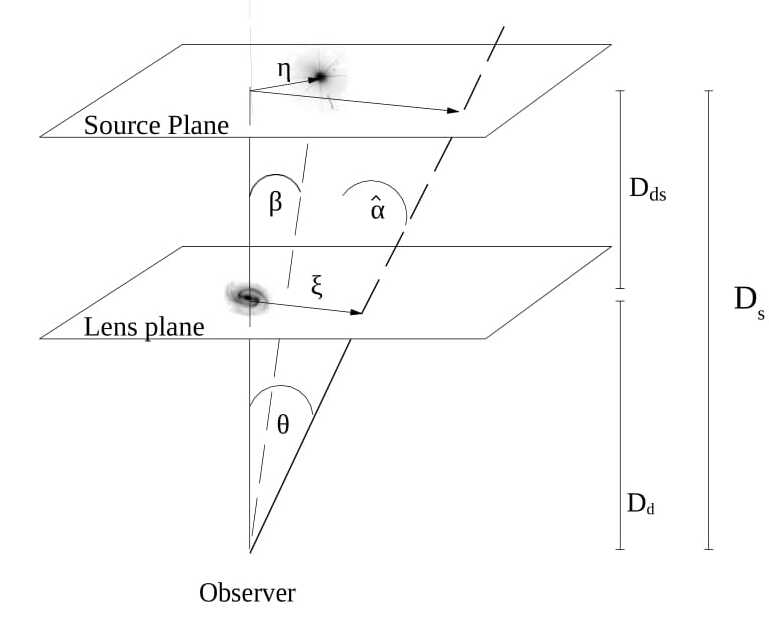
\includegraphics[width=0.5\linewidth]{./figs/lensing.png}
  	\caption{Schematic diagram of the gravitational lensing system~\cite{wiki}.}%
  	\label{fig:lensing}
  \end{figure}
  
  \subsubsection{Lens Equation}
 For a given source, the lens equation is given by,
  
\begin{equation}
\beta =\theta -\alpha (\theta)
\label{LEquation}
\end{equation}
\noindent
Where, $\theta$ be the apparent angular position of the source in the sky, $\beta$ is its true position, and $\alpha $ is the scaled deflection angle.

The angles can be related to the physical distances as,
\begin{equation}
\eta = \frac{D_{s}}{D_{d}}\xi - D_{ds} \hat\alpha(\xi)
\label{AReation}
\end{equation}
\noindent
With, $ D_{d}\theta= \xi $, $ \eta=D_{s}\beta $, and $\hat{\alpha}$ is the true deflection angle which is related to the scaled deflection angle via:
\begin{equation}
\hat\alpha(\xi)=\frac{4G}{c^2}\int d^2{\xi'}\sum(\xi') \frac{\xi-\xi'}{{\mid\xi-\xi'\mid}^2}
\end{equation} 
Where, $\sum(\xi') $ is the surface mass density and $\mid \xi -\xi'\mid$ is the impact parameter for $\sum(\xi') $.
Now, we can define a dimensionless surface mas density with convergence as,
\begin{equation}
\kappa(\theta)=\frac{\sum(D_{d}\theta)}{\sum_{cr}}
\label{Equ:KTheta}
\end{equation}
with the critical surface mass density,
 \begin{equation}
 \Sigma{cr}=\frac{c^2}{4\pi G}\frac{D_{s}}{D_{d}D_{ds}}
 \label{SumCr}
 \end{equation}
 
Now, on rewriting the expression for scaled deflection angle,
\begin{equation}
\alpha(\theta)=\frac{1}{\pi}\int d^2 \theta'_{\kappa}(\theta')\frac{\theta-\theta'}{\mid \theta -\theta'\mid ^2}
\label{ScaledDA}
\end{equation} 
Along with this we also have to define a deflection potential which is to gives information about the mass distribution of the lens is as follow,
\begin{equation}
\psi(\theta)=\frac{1}{\pi}\int d^2\theta'_{\kappa}(\theta')In \mid \theta-\theta'\mid 
\label{psiTheta}
\end{equation}
The use of this quantity is motivated because it encloses all information of the mass distribution of the lens. By means of the deflection potential the following relations can be derived:

\begin{equation}
\alpha(\theta)=\bigtriangledown\psi(\theta)
\label{Equ:AlphaTheta}
\end{equation}
For a better understanding further reading of the references is advised. From the deflection potential a further scalar function, the Fermat potential, can be derived:
\begin{equation}
\tau(\theta; \beta)=\frac{1}{2}(\beta -\theta)^2 -\psi(\theta)
\label{Equ:Format}
\end{equation}

Finally to find the magnification of the images, which is the ratio of a lens to un-lensed flux, is given by
\begin{equation}
\mu =(det A)^{-1}
\end{equation}
Where, \text{A} is the Jacobian matrix of lens mapping

\begin{equation}
A_{ij}=\frac{\partial\beta_{i}}{\partial \theta_{j}}
\end{equation}
\\
\subsubsection{The SIS (Singular Isothermal Sphere)}
A simple model to describe the mass distribution of a galaxy acting as a lens is the singular isothermal sphere (SIS):
\begin{equation}
\rho(r)=\frac{\sigma_{v}^{2}}{2\pi G r^2}
\label{equ:SIS}
\end{equation}
Where $ \sigma^2_{v} $ is the velocity dispersion. Integration along the line of sight yields the surface mass density
\begin{equation}
\Sigma(\xi)=\frac{\sigma^2_{v}}{2G\xi}
\label{equ:Sigma(xi)}
\end{equation}

\noindent
A characteristic angular scale of an axisymmetric lens is given by the Einstein radius $ \theta_{E} $ , defined as the angle inside which the mean of the convergence is unity. As a consequence, the projected mass inside $ \theta_{E} $ can be written as,
\begin{equation}
M(\theta \le \theta_{E})=\pi \theta^2_{E}D^2_{d}\Sigma_{cr}
\end{equation}

For an SIS the Einstein radius reads
\begin{equation}
\theta_{E}=4\pi\bigg( \frac{\sigma_{v}}{c}\bigg)^2\frac{D_{ds}}{D_{s}}
\label{Equ:ThetaE}
\end{equation}
